\documentclass[11pt, english]{article}
\usepackage{graphicx}
\usepackage[colorlinks=true, linkcolor=blue]{hyperref}
\usepackage[english]{babel}
\selectlanguage{english}
\usepackage[utf8]{inputenc}
\usepackage[svgnames]{xcolor}

\usepackage{amsmath}
\usepackage{amsthm}
\usepackage{mathtools}
\usepackage{eucal}
\usepackage{amssymb}
\usepackage{mathrsfs}

\usepackage{listings}
\usepackage{afterpage}
\pagestyle{plain}

\definecolor{dkgreen}{rgb}{0,0.6,0}
\definecolor{gray}{rgb}{0.5,0.5,0.5}
\definecolor{mauve}{rgb}{0.58,0,0.82}

\lstset{frame=tb,
language=Python,
aboveskip=3mm,
belowskip=3mm,
showstringspaces=false,
columns=flexible,
numbers=none,
keywordstyle=\color{blue},
numberstyle=\tiny\color{gray},
commentstyle=\color{dkgreen},
stringstyle=\color{mauve},
breaklines=true,
breakatwhitespace=true,
tabsize=3
}

\usepackage{here}
\usepackage{bm}


\textheight=21cm
\textwidth=17cm
\oddsidemargin=0cm
\pagestyle{plain}

\usepackage{color}
\usepackage{indentfirst}
\usepackage{ragged2e}

% Expectation symbol
\DeclareMathOperator*{\E}{\mathbb{E}}

\global\let\date\relax
\newcounter{unomenos}
\setcounter{unomenos}{\number\year}
\addtocounter{unomenos}{-1}
\stepcounter{unomenos}
\gdef\@date{ \arabic{unomenos} }

\usepackage[backend=bibtex,style=phys]{biblatex}
\bibliography{references} 

\begin{document}

\begin{titlepage}

\begin{center}
Wigner Research Center for Physics, Hungarian Academy of Sciences - \@date\\
\vspace*{0.15in}
Computational Systems Neuroscience Lab \\
\vspace*{0.4in}
\rule{100mm}{0.1mm}\\
\vspace*{0.3in}
\begin{Large}
\textbf{Modelling of the visual cortex with \\ the methods of machine learning} \\
\end{Large}
\vspace*{0.3in}
\rule{100mm}{0.1mm}\\
\vspace*{0.4in}
\begin{large}
Alex Olar \\
\end{large}
\vfill

\includegraphics[width=2cm]{logoFAC.png}
\end{center}
\end{titlepage}

\newcommand{\CC}{C\nolinebreak\hspace{-.05em}\raisebox{.4ex}{\tiny\bf +}\nolinebreak\hspace{-.10em}\raisebox{.4ex}{\tiny\bf +}}
\def\CC{{C\nolinebreak[4]\hspace{-.05em}\raisebox{.4ex}{\tiny\bf ++}}}

\renewcommand{\thesection}{\Roman{section}.}
\renewcommand{\thesubsection}{\Roman{section}. \arabic{subsection}.}
\renewcommand{\thesubsubsection}{\Roman{section}. \arabic{subsection}.\arabic{subsection}.}

\tableofcontents
\newpage

\section{Introduction}

\vspace{7mm}

\subsection{General}

\vspace{5mm}

\par  The visual cortex is a many layered unit in the brain, in which the first computational layer (V1) is known to detect edges in visual stimuli.
The second computational layer is doing further abstraction but we do not yet
have proper information about its role in vision \cite{ZiembaV2}. For the sake of acquiring a
better understanding of the visual representation of the brain, it is crucial to be able to build models that are on one hand not similar in every regard to the brain but on the other hand reproduce its properties, responses to visual input.

\vspace{3mm}

\par Since the brain is capable of behaving generatively, such as imagining things that do not exist from memory, therefore we should aim for developing such models. In this aspect, the latent representational models proved to be very good candidates as the actively researched variational autoencoders (VAE) from the domain of deep learning \cite{kingma2013auto}. This model attempts to represent high-dimensional images in a smaller vector space with auxiliary constraints on the latent representation using deep neural networks.

\subsection{Motivation}

\vspace{5mm}

\par The selection of this topic was motivated by the substantial development in neurobiology that could be achieved with the use and development of deep learning models. We could gather higher level information about the image-processing of the brain. It is important to mention that this research is on the border of different sciences such as information technology and neurobiology consequently it poses an exciting challenge to understand.

\newpage

\section{Models}

\vspace{7mm}

\subsection{Early models}

\vspace{5mm}

\par It was the work of Olshausen and Field \cite{olshausen1996emergence} who proposed a model describing the structure of the first layer in the visual cortex (V1). The main assumption than an image $I(x, y)$ can be decomposed on a set of linear basis functions:

\vspace{3mm}

\begin{equation}
    I(x, y) = \sum_{i}a_i \Phi_{i}(x, y)
\end{equation}

\vspace{3mm}

\par Where the components $a_{i}$ are decorrelated pairwise $\E (a_i a_j) = \E a_i \E a_j$. These assumptions were made to satisfy three main point:

\vspace{3mm}

\begin{itemize}
    \item spatially localized
    \item oriented
    \item bandpass - selective to structures at different scaled
\end{itemize}

\vspace{3mm}

\par PCA \footnote{Pricipal Component Analysis} was not fit for this type of problem since it provides a good tool for describing data where pairwise linear correlations are the most important form of statistical dependence. However, it is not the case for high-order correlations in natural images. In order to capture this they proposed a solution that minimizes entropy while sparsely coding the natural images, meaning that they wanted to describe each via a small set of variables out of the large set. The method developed is called sparse coding and a special case of it is ICA \footnote{Independent Component Analysis - \url{https://redwood.berkeley.edu/wp-content/uploads/2018/08/sparse-coding-ICA.pdf}}.

\subsection{VAE}

\vspace{5mm}

\par Autoencoders are mostly used to reduce dimensionality of data in an unsupervised manner. They consist of an encoder and a decoder model surrounding the reduced representation. These models are usually realized as neural networks due to their generalization capability. Autoencoders are a crucial tool for data compression and can reach better results than traditional tools \cite{theis2017lossy}. Variational autoencoders tackle the same problem while constraining the latent, reduced representation. This sacrifices reconstruction accuracy in order to learn a better representation of the dataset.

\subsubsection{Math}

\par Considering a dataset $\boldsymbol{X} = \big\{\boldsymbol{\bm{x}}^{i}\big\}_{i = 1}^{N}$ that consists of independently and identically distributed samples of an underlying distribution it can be assumed that the data has some underlying, unobserved variable $\boldsymbol{\bm{z}}$. The value $\boldsymbol{\bm{z}}^{i}$, corresponding to a sample $\boldsymbol{\bm{x}}^{i}$, is first generated from a prior distribution $p_{\boldsymbol{\vartheta_{real}}}(\boldsymbol{\bm{z}})$ and $\boldsymbol{\bm{x}}^{i}$ is then generated from a conditional distribution $p_{\vartheta_{real}}(\boldsymbol{\bm{x}} | \boldsymbol{\bm{z}})$. Since the real model parameters $\vartheta_{real}$ are unknown we can only approximate them with the encoder and decoder parametric models.
\par We want to approximate the posterior probability:

\vspace{3mm}

\begin{equation}
    p_{\boldsymbol{\vartheta}}(\boldsymbol{\bm{z}} | \boldsymbol{\bm{x}}) \propto p_{\boldsymbol{\vartheta}}(\boldsymbol{\bm{x}} | \boldsymbol{\bm{z}}) p_{\boldsymbol{\vartheta}}(\boldsymbol{\bm{z}})
\end{equation}

\vspace{3mm}

\par Where basically we just applied Bayes-theorem for the likelihood and the prior to acquire the posterior. We build an encoder/recognition model $q_{\phi}(\boldsymbol{\bm{z}} | \boldsymbol{\bm{x}})$ and a decoder model $p_{\vartheta}(\boldsymbol{\bm{x}} | \boldsymbol{\bm{z}})$. The probabilistic encoder produces a distribution over $\boldsymbol{\bm{z}}$ that should properly approximate the prior while the  decoder provides samples from the approximated true distribution given a latent code. This is obviously a two-step generation process. 

\vspace{3mm}

\par In the article of Kingma and Welling \cite{kingma2013auto} they present a variational model that can be trained with gradient descent including stochastic variables. They achieve this in detail as follows:

\vspace{3mm}

\begin{gather*}
    recognition\ model\ :\  q_{\phi}(\bm{z}|\bm{x}) \xrightarrow{\text{approximates}} p_{\vartheta_{real}}(\bm{z} | \bm{x}) \\
    probabilistic\ decoder\ :\ p_{\theta}(\bm{x} | \bm{z}) \xrightarrow{\text{approximates}} p_{\theta_{real}}(\bm{x} | \bm{z})
\end{gather*}

\vspace{3mm}

\par As the data points from the dataset are independent $p(\bm{x}^{(1)}, \bm{x}^{(2)}, ..., \bm{x}^{(N)}) = p(\bm{x}^{(1)})p(\bm{x}^{(2)})\cdot ... \cdot p(\bm{x}^{(N)})$ and applying that $p(\bm{x}^{(i)})$, so approximating $p(\bm{x}^{(i)})$ in general:

\vspace{3mm}

\begin{gather}
    \ln(p(\bm{x}^{(i)})) = \ln\int p(\bm{x}^{(i)}, \bm{z})dz \quad from\ marginal\ prob.\ dist.\\
    \ln(p(\bm{x}^{(i)})) = \ln\int p(\bm{x}^{(i)}, \bm{z})\frac{q(\bm{z})}{q(\bm{z})}dz \quad introducing\ the\ prior \\
    \ln(p(\bm{x}^{(i)})) = \ln \E_{q(\bm{z})} \Big( \frac{p(\bm{x}^{(i)}, \bm{z})}{q(\bm{z})}\Big) \\
    \ln \E_{q(\bm{z})} \Big( \frac{p(\bm{x}^{(i)}, \bm{z})}{q(\bm{z})}\Big) \geq \E_{q(\bm{z})} \ln\Big( \frac{p(\bm{x}^{(i)}, \bm{z})}{q(\bm{z})}\Big) \quad applying\ Jensen's\ inequality \\
    L_{i} = \ln(p(\bm{x}^{(i)})) \geq \E_{q(\bm{z})} \ln\Big( \frac{p(\bm{x}^{(i)}, \bm{z})}{q(\bm{z})}\Big) \quad ELBO
\end{gather}

\vspace{3mm}

\par Jensen's inequality holds for convex functions and the natural logarithm is such. By applying the definition of the joint probability term $p(\bm{x}, \bm{z}) = p(\bm{x} | \bm{z})p(\bm{z})$ and realizing that we use the recognition model for $q(\bm{z})$ in our case $q_{\phi}(\bm{z} | \bm{x})$:

\vspace{3mm}

\begin{equation}
    L_{i} \geq \E_{q_{\phi}(\bm{z} | \bm{x})} \Big( \ln p(\bm{x}^{(i)} | \bm{z}) \Big) + \E_{q_{\phi}(\bm{z} | \bm{x})} \Big( \ln p_{\theta}(\bm{z} | \bm{x}^{(i)}) \Big) - \E_{q_{\phi}(\bm{z} | \bm{x})} \Big( \ln q_{\phi}(\bm{z} | \bm{x}^{(i)}) \Big)
\end{equation}

\vspace{3mm}

\par By introducing the Kullback-Leibler-divergence term:

\vspace{3mm}

\begin{gather*}
    KL(q_{\phi}(\bm{z} | \bm{x}^{(i)}) | p_{\theta}(\bm{z} | \bm{x}^{(i)})) = \int q_{\phi}(\bm{z} | \bm{x}^{(i)})\ln \frac{q_{\phi}(\bm{z} | \bm{x}^{(i)})}{p_{\theta}(\bm{z} | \bm{x}^{(i)})}dz = \E_{q_{\phi}(\bm{z} | \bm{x}^{(i)})} \Big( \ln \frac{q_{\phi}(\bm{z} | \bm{x}^{(i)})}{p_{\theta}(\bm{z}|\bm{x}^{(i)})}  \Big) \\ \\
    KL(q_{\phi} | p_{\theta}) = -L_{i} + \E_{q_{\phi}(\bm{z} | \bm{x}^{(i)})} \Big( \ln p_{\theta}(\bm{x}^{(i)} | \bm{z}) \Big) \quad using\ Bayes-theorem
\end{gather*}

\vspace{3mm}

\par The goal of the algorithm is to optimize the variational lower bound (ELBO) with respect to the parameters $\phi, \theta$. We also introduce $p_{\theta}(\bm{z} | \bm{x}^{(i)}) \equiv p_{\theta}(\bm{z})$, for all data points, as our prior distribution over the latent variables. Since the gradient of the ELBO is a bit problematic, especially requiring a large amount of computation w. r. t. $\phi$ Kingma and Welling came up with auto-encoding variational Bayes (AEVB) algorithm that makes the model trainable via stochastic gradient descent.

\paragraph{The reparametrization trick \newline \newline}

\par Let $\bm{z}$ be a random variable sampled from $   q_{\phi}(\bm{z} | \bm{x})$. It is often possible to express \footnote{1. tractable CDF, 2. norm-scale functions, 3. composition} such variable as a deterministic mapping $\bm{z} = g_{\phi}(\bm{\epsilon}, \bm{x})$ where $\bm{\epsilon}$ is an independent random variable with marginal distribution $p(\bm{\epsilon})$. Since we know from basic probability theory $q_{\phi}(\bm{z} | \bm{x})dz = p(\bm{\epsilon})d\bm{\epsilon}$. Therefore the expected value of a function $f(\bm{z})$ can be computed as:

\vspace{3mm}

\begin{equation}
    \int f(\bm{z})q_{\phi}(\bm{z} | \bm{x}^{(i)})dz = \int p(\bm{\epsilon})f(g_{\phi}(\bm{\epsilon}, \bm{x}^{(i)})) d\bm{\epsilon} \approx \frac{1}{L}\sum_{l=1}^{L}f(g_{\phi}(\bm{\epsilon}^{(l)}, \bm{x}^{(i)}))
\end{equation}

\vspace{3mm}

\par Where $\bm{\epsilon}^{(l)}$ is sampled from $p(\bm{\epsilon})$. If we take $q_{\phi}(\bm{z} | \bm{x})$ as the Gaussian distribution $\bm{z} \sim N(\mu, \sigma)$ then a straightforward reparametrization $g_{\phi}$ occurs as $\bm{z} = \mu + \bm{\epsilon} \sigma$.

\vspace{3mm}

\begin{figure}[H]
    \centering
    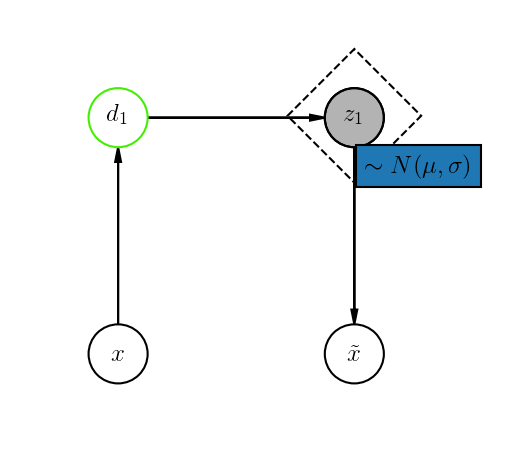
\includegraphics[width=0.4\textwidth]{vae.png}
    \caption{Variational autoencoder}
    \label{fig:vae}
\end{figure}

\vspace{3mm}

\par As we can see in figure \ref{fig:vae} the variational autoencoder is outlined. The general intuition is that a neural network approximates $q_{\phi}(\bm{z} | \bm{x})$ over that dataset and it is assumed that it takes a multivariate Gaussian form for the true, intractable posterior $p_{\theta_{real}}(\bm{z} | \bm{x})$.

\vspace{3mm}

\par We sample $\bm{z}$ from a Gaussian where the mean and standard deviation is the output of the probabilistic encoder and than we apply the reparametrization. With this method the variational lower bound becomes simple to approximate:

\vspace{3mm}

\begin{equation}
    L_{i} \simeq \frac{1}{2}\sum_{j = 1}^{J}\Big( 1 + \ln(\sigma^{(i)}_{j})^{2} - (\mu^{(i)}_{j})^{2} - (\sigma^{(i)}_{j})^{2} \Big) + \frac{1}{L}\sum_{l=1}^{L}\ln p_{\theta}(\bm{x}^{(i)} | \bm{z}^{(i, l)})
\end{equation}

\vspace{3mm}

\par Where $\bm{z}^{(i, l)} = \mu^{(i)} + \sigma^{(i)} \odot \bm{\epsilon}^{(l)}$ where $\mu, \sigma$ come from $q_{\phi}(\bm{z} | \bm{x})$ and $\bm{\epsilon}$ from $p(\bm{\epsilon}) \sim N(0, 1)$. The first part is the Kullback-Leibler-divergence between a unit Gaussian and $N(\mu^{(i)}, \sigma^{(i)})$ Gaussian, this can be analytically calculated.

\vspace{3mm}

\par In practice this means that the KL-divergence can be computed efficiently after encoding and to speed up the process $L = 1$ is usually chosen to not to pass the code through the decoder several times. In the case of continuous pixel values the second part of the ELBO can be approximated with a multivariate Gaussian whereas in case of binary pixel values it becomes a Bernoulli-distribution. 

\vspace{3mm}

\par The models were built in Keras \cite{chollet2015keras} and using its built-in visualization tool I was able to show how my VAE is built:

\vspace{3mm}

\begin{figure}[H]
    \centering
    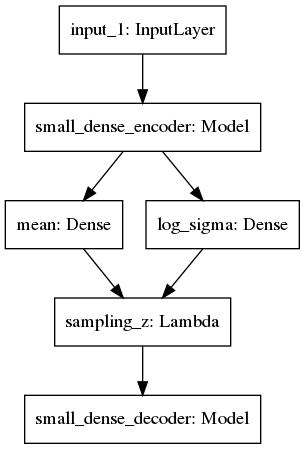
\includegraphics[width=0.4\textwidth]{vae_keras.png}
    \caption{Variational autoencoder implementation in Keras}
\end{figure}

\vspace{3mm}

\par It is a bit confusing since the arrows only mean parameter passes here not dependence as in the graphical representation where the nodes of the graph are random variables as opposed to models. 

\subsection{LVAE}

\vspace{5mm}

\par The ladder variational autoencoder was first introduced in 2016 \cite{sonderby2016ladder} one year after the UNET \cite{ronneberger2015u} architecture which used ladder like parameter sharing across encoding and decoding layers. Using ladder like structures became popular around 2015.

\vspace{3mm}

\par I need to emphasise that the LVAE model only differs from the VAE in the inference model $q_{\phi} (z | x)$ by introducing more stochastic layers to provide better reconstruction results and to learn a more abstract latent representation oft the data. In \cite{sonderby2016ladder} they approximated $p_{\theta_{real}}$ by splitting it up two L layers:

\vspace{3mm}

\begin{equation}
    p_{\theta_{real}}(\bm{z}) =  p_{\theta}(\bm{z}_{L})\prod_{i = 1}^{L - 1}p_{\theta}(\bm{z}_i | \bm{z}_{i+1})
\end{equation}

\vspace{3mm}

\par In practice I added one additional layer to the VAE architecture as they did in the above mentioned article. Here:

\vspace{3mm}

\begin{gather*}
    p_{\theta}(\bm{z}_L) = N(\bm{z}_L  ~ | ~ 0, 1) \quad called\ \epsilon\ previously\\
    p_{\theta}(\bm{z}_i ~ | ~ \bm{z}_{i+1}) = N(\bm{z}_i ~ |  ~ \mu_{p,i}(\bm{z}_{i+1}), \sigma_{p, i}(\bm{z}_{i+1}))
\end{gather*}

\vspace{3mm}

\par Of course, I outlined here the case of continuous variables the case where the dataset is not binarized. 

\vspace{3mm}

\begin{figure}[H]
    \centering
    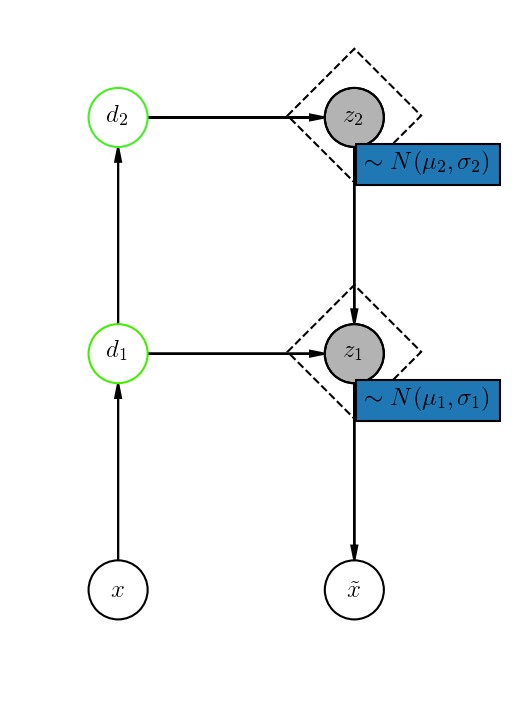
\includegraphics[width=0.5\textwidth]{lvae.png}
    \caption{Ladder variational autoencoder}
\end{figure}

\vspace{3mm}

% TODO: change figure
\par The models were built with Keras \cite{chollet2015keras} as well:

\vspace{3mm}

\begin{figure}[H]
    \centering
    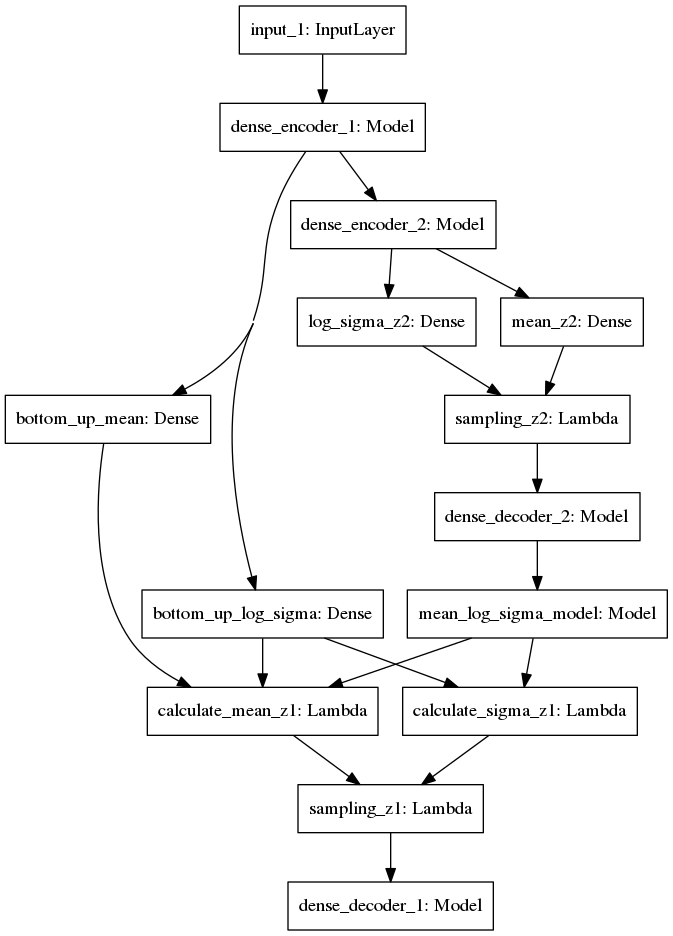
\includegraphics[width=0.65\textwidth]{dense_lvae_keras.png}
    \caption{Ladder variational autoencoder implementation in Keras}
    \label{fig:keras_lvae}
\end{figure}

\vspace{3mm}

\par Keras provides high modularity so the blocks \textit{dense\_encoder\_1, dense\_decoder\_1, etc.} can all be
changed and swapped to higher or lower capacity models with MLP or convolutional architectures.

\newpage

\section{Datasets}

\vspace{7mm}

\par Mainly I used synthetically generated texture families with my models that resemble the Simonchelli-Portilla texture family \cite{portilla2003image} but I experimented with the MNIST, Fashion-MNIST \cite{xiao2017fashion}, CIFAR-10, natural textures and the dSprites dataset \cite{matthey2017dsprites}. I wanted to find out whether it would be possible for a latent variable model to disentangle parameters such as contrast from images.

\vspace{7mm}

\section{Implementation details}

\vspace{7mm}

\par I used the $\beta-$VAE and ($\beta-$)LVAE architectures as I mentioned. From the original LVAE article \cite{sonderby2016ladder} I used incremental $\beta$ learning, meaning that I raised my $\beta$ value incrementally during learning for 3/7ths of the epochs and kept on learning with $\beta = \beta_{max}$ for the remaining steps. From this article I also tested batch-normalization and built modular models that include convolution with batch-normalization as well. The value $\beta_{max}$ can be set before the start of the training, $\beta_{max} = 1$ is the case of the VAE but raising its value directly emphasizes the influence of the KL-term during training.

\vspace{3mm}

\par For both of my latent variable model architectures (VAE, LVAE) I use the reparametrization trick on the deepest variational parameter to be able to later on sample from zero centered unit Gaussian:

\vspace{3mm}

\begin{equation}
    \boldsymbol{\bm{z}}^{(i, l)} = \boldsymbol{\mu}^{(i)} + \boldsymbol{\sigma}^{(i)} \odot \boldsymbol{\bm{\epsilon}}^{(l)}
\end{equation}

\vspace{3mm}

\par Where $\boldsymbol{\bm{\epsilon}}^{(l)} \sim \boldsymbol{N}(0, 1)$ in order to be able to achieve that when sampling from the generative model we would only need to sample this $\bm{\epsilon}$ parameter and feed it to the network to generate learnt representations corresponding to this latent random variable.

\vspace{3mm}

\par Both models can be sampled after training. However, in the VAE architecture it is straightforward to do so, on the other hand, the LVAE needs bottom up information from the image since the calculation of the mean and standard deviation is deterministic from the generated bottom up (from the input image - referenced as BU) and top down (from the stochastic latent parameter - referenced as TD) components:

\vspace{3mm}

\begin{gather*}
    \hat{\sigma}_{1} = \frac{1}{\sigma_{BU}^{-2} + \sigma_{TD}^{-2}} \\ \\
    \hat{\mu}_{1} = \frac{\mu_{BU}\sigma_{BU}^{-2} + \mu_{TD}\sigma_{TD}^{-2}}{\sigma_{BU}^{-2} + \sigma_{TD}^{-2}}
\end{gather*}

\vspace{3mm}

\par When sampling $\bm{z}^{(2)}$, the deepest latent vector, the bottom up standard deviation is considered infinite, therefore:

\vspace{3mm}

\begin{equation*}
    \hat{\sigma}_{1} = \sigma_{TD}^{2} \quad \quad \hat{\mu_{1}} = \mu_{TD}
\end{equation*}

\vspace{3mm}

\par This provides a good way of examining the trained models. Doing a full reconstruction and comparing the bottom up means and standard deviations with the top down means and standard deviations we can find out which of these have a bigger influence on the reconstruction. It might be that we only add noise to the generated images with the stochasticity from the deepest latent sampling and only the bottom up components are used for reconstruction, I explore this more in a later section.

\vspace{3mm}

\par My implementation consists mostly dense layers and rectified linear units. Basically each unit of the two-unit ladder encoder includes an MLP in the LVAE architecture. Also, I experimented with convolutional and deconvolutional \footnote{referred to also as transpose convolution, inverse convolution} encoders and decoders for both the VAE and LVAE architectures. Not only did I create variational/stochastic models but also I implemented autoencoders with no restriction on the latent space for comparison.

\vspace{3mm}

\par In \ref{fig:vae}, \ref{fig:keras_lvae} it can be spotted that there is an intermediate step included in the generation process of the standard deviations. Since linear layers are constructing the means and the standard deviations they are not restricted to be positive which is not an issue for the means of Gaussian distributions but for the standard deviations. It is usually resolved as generating the logarithm of the standard deviations and then taking their exponential each time their value is needed.

\vspace{3mm}

\par As I mentioned during the description of the models used, I implemented everything in the framework Keras and used the package $\bm{tensorflow\_probability}$ to be able to include statistical methods, such as probability distribution sampling in my code. In addition, I want to emphasize that I have build a Python library out of my code to provide a framework to test variational autoencoders with different datasets. The package is available via $\bm{pip}$ \footnote{\url{https://pypi.org/project/csnl-vae-olaralex/}} and the corresponding datasets to use with some example Jupyter notebooks are available through Kaggle \footnote{\url{https://www.kaggle.com/dumbo666/wigner-csnl-textures-mnist-format}}.

\newpage
\printbibliography

\end{document} 